\documentclass[a4paper,11pt]{article}

\usepackage[T1]{fontenc}
\usepackage[utf8]{inputenc}
\usepackage{graphicx}
\usepackage{xcolor}
\usepackage{caption}
\usepackage{subcaption}

\usepackage{tgtermes}

\usepackage[
pdftitle={Statistical Machine Learning}, 
pdfauthor={Inez Wijnands \& Guido Zuidhof, Radboud University Nijmegen},
colorlinks=true,linkcolor=blue,urlcolor=blue,citecolor=blue,bookmarks=true,
bookmarksopenlevel=2]{hyperref}
\usepackage{amsmath,amssymb,amsthm,textcomp}
\usepackage{enumerate}
\usepackage{multicol}
\usepackage{tikz}

\usepackage{geometry}
\geometry{total={210mm,297mm},
left=25mm,right=25mm,%
bindingoffset=0mm, top=20mm,bottom=20mm}


\linespread{1.3}

\newcommand{\linia}{\rule{\linewidth}{0.5pt}}

% custom theorems if needed
\newtheoremstyle{mytheor}
    {1ex}{1ex}{\normalfont}{0pt}{\scshape}{.}{1ex}
    {{\thmname{#1 }}{\thmnumber{#2}}{\thmnote{ (#3)}}}

\theoremstyle{mytheor}
\newtheorem{defi}{Definition}

% my own titles
\makeatletter
\renewcommand{\maketitle}{
\begin{center}
\vspace{2ex}
{\huge \textsc{\@title}}
\vspace{1ex}
\\
\linia\\
\@author  \@date
\vspace{4ex}
\end{center}
}
\makeatother
%%%

% custom footers and headers
\usepackage{fancyhdr,lastpage}
\pagestyle{fancy}
\lhead{}
\chead{}
\rhead{}
\lfoot{Assignment \textnumero{} 1}
\cfoot{}
\rfoot{Page \thepage\ /\ \pageref*{LastPage}}
\renewcommand{\headrulewidth}{0pt}
\renewcommand{\footrulewidth}{0pt}
%

% code listing settings
\usepackage{listings}
\lstset{
    language=Python,
    basicstyle=\ttfamily\small,
    aboveskip={1.0\baselineskip},
    belowskip={1.0\baselineskip},
    columns=fixed,
    extendedchars=true,
    breaklines=true,
    tabsize=4,
    prebreak=\raisebox{0ex}[0ex][0ex]{\ensuremath{\hookleftarrow}},
    frame=lines,
    showtabs=false,
    showspaces=false,
    showstringspaces=false,
    keywordstyle=\color[rgb]{0.627,0.126,0.941},
    commentstyle=\color[rgb]{0.133,0.545,0.133},
    stringstyle=\color[rgb]{01,0,0},
    numbers=left,
    numberstyle=\scriptsize\ttfamily,
    stepnumber=1,
    numbersep=10pt,
    captionpos=t,
    escapeinside={\%*}{*)}
}

%%%----------%%%----------%%%----------%%%----------%%%

\begin{document}

\title{Statistical Machine Learning \\ Assignment 1}

\author{Inez Wijnands (s4149696) \& Guido Zuidhof (s4160703)\\ Radboud University Nijmegen\\}

\date{29/09/2015}

\maketitle

\section*{Exercise 1}
\textit{The entire code listing is in a separate file. The listings shown here are merely code snippets}.
\begin{enumerate}
\item The function $t = f(x)$ we have created is $f(x) = 1 + sin(8x+1)$. This function is neither even nor odd. An even function is a function such as $cos(x)$, and an odd function is a function such as $sin(x)$, since we changed the phase and intercept of $sin(x)$ our function is neither. See Figure 1 for the function $f(x)$ and observations $\mathcal{D}$. \vspace{-0.5cm}\begin{figure}[h]
\centering
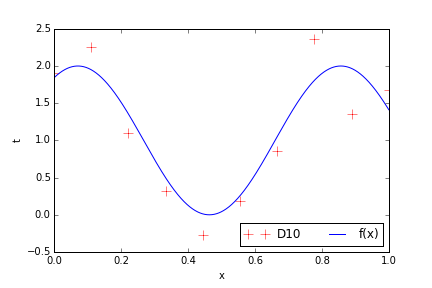
\includegraphics[scale=0.8]{1_1.png}\vspace{-0.5cm}
\caption{\vspace{-0.2cm}The function $f(x)$ and observations $\mathcal{D}$ are plotted (similar to Bishop, Fig.1.2)}
\end{figure}
\item See Listing 1 for the function $\boldsymbol{w} = PolCurFit(\mathcal{D},M)$.\vspace{-0.5cm}
\begin{lstlisting}[label={list:first},caption=Python code for function PolCurFit -- Input are the observations $\mathcal{D}$ and the results $t$ of function $f(x)$ and the order of the polynomial $M$. The functions calculates the $A$-matrix and $T$-vector and solves this equation to find the weights.]
def PolCurFit(D,M):
    x = D[0]
    t = D[1]
    M = M + 1
    A = np.array([[Aij(i,j,x) for j in xrange(M)] for i in xrange(M)])
    T = np.array([Ti(i,t,x) for i in xrange(M)])
    return np.linalg.solve(A,T)
\end{lstlisting}
\item See Figure 2 \& 3 \vspace{-0.5cm}\begin{figure}[h]
\centering
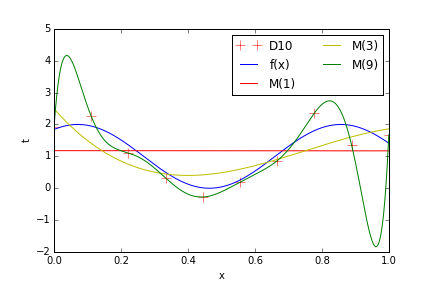
\includegraphics[scale=0.8]{1_2_10.png}\vspace{-0.5cm}
\caption{\vspace{-0.2cm} In this figure, the observations $\mathcal{D}$, the function $f(x)$ and polynomials of different orders of $M$ are shown.}
\end{figure}
\vspace{-0.5cm}\begin{figure}[h]
\centering
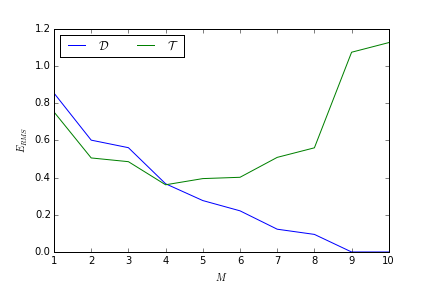
\includegraphics[scale=0.8]{1_3_10.png}\vspace{-0.5cm}
\caption{\vspace{-0.2cm} For the various orders $M = [1,\hdots,10]$ and for each solution $\boldsymbol{w}^*$ the root-mean-quare error $E_{RMS} = \sqrt{2E(\boldsymbol{w}^*)/N}$ is computed of the corresponding polynomial, evaluated on both the training set $\mathcal{D}$ and the testset $\mathcal{T}$ (similar to Bishop, Fig.1.5)}
\end{figure}
\item 
\item
\end{enumerate}

\section*{Exercise 2}
\begin{enumerate}
\item Simplify:\\
$h(x,y) = 100(y - x^2)^2 + (1 - x)^2 = 100(y^2 - 2x^2y + x^4) + x^2 - 2x + 1 =$ \\
$100y^2 - 200x^2y + 100x^4 + x^2 - 2x + 1$\\
\vspace{0.4cm}
Derive:\\
$\frac{dh(x,y)}{dx} = - 400xy + 400x^3 + 2x - 2$\\
$\frac{dh(x,y)}{dy} = 200y - 200x^2$\\
\vspace{0.4cm}
Set derivative of $h(x,y)$ equal to zero:\\
$200y - 200x^2 = 0 \rightarrow 200y = 200x^2 \rightarrow y = x^2$\\
$- 400xy + 400x^3 + 2x - 2 = 0 \rightarrow$ use $y = x^2$ $\rightarrow 400x^3 = 400x^3 + 2x - 2 \rightarrow 2x = 2 \rightarrow x = 1$\\
$y = x^2$ and $x = 1 \rightarrow y = 1^2 = 1$\\
(1,1) is the minimum of $h(x,y)$
\item
\end{enumerate}

\section*{Exercise 3}


\end{document}
